\documentclass[11pt,a4paper]{article}

% Packages
\usepackage[margin=2.2cm]{geometry}
\usepackage[T1]{fontenc}
\usepackage[utf8]{inputenc}
\usepackage{lmodern}
\usepackage{textcomp}
\usepackage{microtype}
\usepackage{enumitem}
\usepackage{xcolor}
\usepackage{graphicx}
\usepackage{booktabs}
\usepackage{tabularx}
\usepackage{tikz}
\usetikzlibrary{positioning,arrows.meta}
\usepackage{hyperref}

\hypersetup{
    colorlinks=true,
    linkcolor=black,
    urlcolor=blue
}

\setlist[itemize]{leftmargin=1.5em, itemsep=2pt}
\setlist[enumerate]{leftmargin=1.8em, itemsep=3pt}
\setlength{\parindent}{0pt}
\setlength{\parskip}{5pt}

% Actual prompts are quoted verbatim, including typos.
\newcommand{\prompt}[1]{\textit{``#1''}}
\newcommand{\repolink}{\url{https://github.com/valentinaAnt/expense-tracker-budget-analyzer}}

\begin{document}

% ==================================================
% TITLE PAGE
% ==================================================

\begin{titlepage}
    \centering

    \vspace*{2cm}

    {\Large\textbf{AI-Assisted Development -- Exam}\par}

    \vspace{1.5cm}

    {\Huge\bfseries Expense Tracker \& Budget Analyzer\par}

    \vspace{0.7cm}

    {\large Project Documentation\par}

    \vspace{2cm}

    \begin{flushleft}
        \textbf{Student:} Valentina Antimova

        \vspace{0.4cm}

        \textbf{AI Development Tool:}
        Claude Code (Visual Studio Code extension, model Claude Opus 5.5)

        \vspace{0.4cm}

        \textbf{Technologies:}
        JavaScript (ES modules), Node.js, Express 5, SQLite (better-sqlite3),
        HTML5, CSS3, vanilla JavaScript, \texttt{node:test}

        \vspace{0.4cm}

        \textbf{GitHub Repository:}
        \repolink

        \vspace{0.4cm}

        \textbf{Submission Date:} \today
    \end{flushleft}

    \vfill

    {\large Academic Project\par}
\end{titlepage}

\pagenumbering{roman}
\tableofcontents
\newpage
\pagenumbering{arabic}

% ==================================================
% 1. PROJECT IDEA AND SYSTEM REQUIREMENTS
% ==================================================

\section{Project Idea and System Requirements}

\subsection{Project Overview}

The \textbf{Expense Tracker \& Budget Analyzer} is a browser-based
personal finance application that helps one person control their
monthly spending. The user records expenses (amount, category, date,
description), sets a monthly spending limit per category, and reviews a
dashboard that shows how much was spent in the selected month, how the
spending is distributed across categories, how much of each budget is
used or exceeded, and which categories cost the most.

The problem it addresses is that spending is often only noticed at the
end of the month. Spreadsheets require manual formulas and give no
warning when a budget is close to its limit. The application runs
locally on Windows with a Node.js and Express backend, a SQLite database
and a plain HTML, CSS and JavaScript interface. It was developed
incrementally with Claude Code as the AI coding assistant.

\subsection{Functional Requirements}

\begin{enumerate}
    \item \textbf{Expense Management:}
    Users can add, view, edit, and delete expenses (deletion requires
    confirmation). Each expense has an amount, category, date, and
    description.

    \item \textbf{Categories and Filtering:}
    Every expense belongs to one category. Nine default categories (Food,
    Transport, Housing, Utilities, Health, Entertainment, Shopping,
    Education, Other) are created with a new database; users can add their
    own, rename them, and delete categories that are no longer used.
    Expenses can be filtered by month (interface and API) and by category
    (API).

    \item \textbf{Financial Dashboard:}
    For a selected month the dashboard shows total spending, the total
    monthly budget, the budget remaining or exceeded, and the number of
    categories over budget.

    \item \textbf{Budget Management:}
    Users can set, change, and remove one recurring monthly limit per
    category. The system marks each category as within budget, close to
    the limit (from 80\,\%), or over budget.

    \item \textbf{Spending Analytics:}
    A CSS bar chart compares spending with each budget, and the three
    highest-spending categories are listed with their share of the
    month's total. All figures are calculated from stored records.

    \item \textbf{Data Persistence:}
    Expenses and budgets are stored in SQLite and remain available after
    the server is restarted.
\end{enumerate}

\subsection{Non-Functional Requirements}

\begin{itemize}
    \item \textbf{Usability:} The interface is responsive (desktop and
    mobile widths), uses labelled form fields, keyboard-accessible
    controls, and announces success and error messages to screen readers.
    Error messages disappear as soon as a field is corrected, and a
    half-filled expense form can be cleared.

    \item \textbf{Reliability:} Money is stored as integer cents, so
    totals are exact. Invalid data is rejected on the server with
    structured JSON errors, and unexpected errors never crash the server.

    \item \textbf{Maintainability:} The code is separated into routes,
    services, validation, error handling, database, and frontend
    modules, with only two runtime dependencies.

    \item \textbf{Security:} All SQL uses parameterized statements; user
    text is rendered with \texttt{textContent}, never as HTML, which
    prevents cross-site scripting; the server listens only on
    \texttt{127.0.0.1}; the database is excluded from Git.

    \item \textbf{Testability:} Business logic and the HTTP API are
    covered by automated tests that use a temporary database, including
    invalid inputs, empty months, month boundaries, and budget limits.
\end{itemize}

\subsection{Scope and Expected Outcome}

The project is a single-user application running locally, without user
accounts, bank integrations, payment processing, income tracking, or
cloud synchronization. The outcome is a functional, tested web
application that demonstrates modular design, persistent data
management, accurate financial calculations, and the practical use of
an AI coding assistant throughout the development lifecycle.

% ==================================================
% 2. SYSTEM ARCHITECTURE
% ==================================================

\section{System Architecture -- Modules}

\subsection{Application Structure}

The application uses a layered architecture in a single repository
(Figure~\ref{fig:architecture}). The browser loads static files served
by Express and communicates with a JSON REST API. Routes only translate
HTTP requests into service calls; services contain validation, business
rules, and parameterized SQL; the database module opens SQLite and
creates the schema. \texttt{createApp(db)} receives the database as a
parameter, so tests can run the real application against a temporary
database.

\begin{figure}[htbp]
\centering
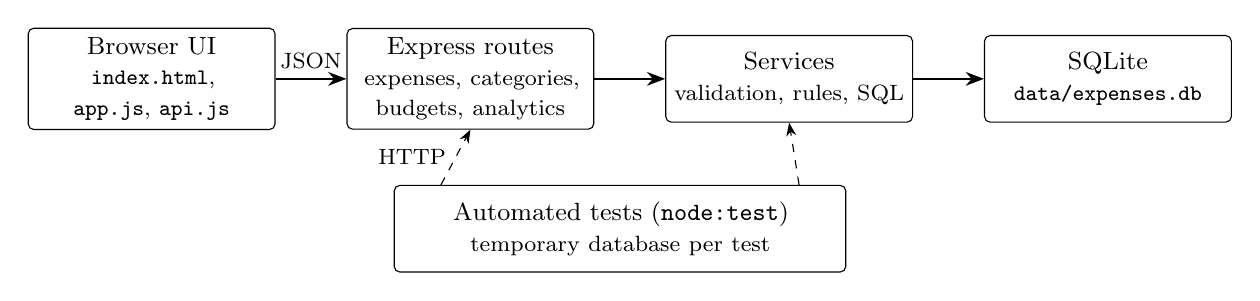
\begin{tikzpicture}[
    box/.style={draw, rounded corners=2pt, align=center, minimum height=1.1cm,
                text width=2.9cm, font=\small},
    arrow/.style={-{Stealth}, thick},
    dashedarrow/.style={-{Stealth}, dashed}]
    \node[box] (ui) {Browser UI\\\footnotesize\texttt{index.html}, \texttt{app.js}, \texttt{api.js}};
    \node[box, right=0.9cm of ui] (routes) {Express routes\\\footnotesize expenses, categories, budgets, analytics};
    \node[box, right=0.9cm of routes] (services) {Services\\\footnotesize validation, rules, SQL};
    \node[box, right=0.9cm of services] (db) {SQLite\\\footnotesize\texttt{data/expenses.db}};
    \node[box, below=0.7cm of routes, xshift=1.9cm, text width=5.5cm] (tests)
        {Automated tests (\texttt{node:test})\\\footnotesize temporary database per test};
    \draw[arrow] (ui) -- node[above, font=\footnotesize]{JSON} (routes);
    \draw[arrow] (routes) -- (services);
    \draw[arrow] (services) -- (db);
    \draw[dashedarrow] (tests.north west) ++(0.6,0) -- node[left, font=\footnotesize]{HTTP} (routes.south);
    \draw[dashedarrow] (tests.north east) ++(-0.6,0) -- (services.south);
\end{tikzpicture}
\caption{Layered architecture; dashed arrows show how the tests access the system.}
\label{fig:architecture}
\end{figure}

\textbf{Technology choices.} Express~5 forwards errors from route
handlers to one central error handler. \texttt{better-sqlite3} (13.0.3)
was chosen over the built-in \texttt{node:sqlite}, which is still marked
experimental, because it is mature, provides prepared statements and
transactions, and ships prebuilt Windows binaries. The tests use the
built-in \texttt{node:test} runner and \texttt{fetch}, so no test
libraries are needed.
The project targets Node.js~24 LTS; the final tests ran on Node.js
24.22.1 with npm 11.19.1 (early development used Node.js~25.8.0).

\subsection{User Interface Module}

\texttt{public/index.html} contains one page with summary cards, a
category bar chart, a top-categories list, the expense form (with
\emph{Clear}/\emph{Cancel}), a categories panel, the budget list, and the
expense table for the selected month. \texttt{api.js} is the only module
that calls \texttt{fetch} and converts error responses into one
\texttt{ApiError} type; \texttt{app.js} renders data, handles events, and
formats amounts as euros (\texttt{Intl.NumberFormat}). A
\texttt{<dialog>} confirms deletions, and a month picker drives every
section. The neutral blue-grey design uses colour only for budget
warnings.

\subsection{Expense Management Module}

\texttt{expenseService.js} validates the complete request and reports
all invalid fields together, then performs create, read, update, delete,
and filtered list operations. \texttt{validation.js} holds shared
checks: amounts are parsed as text into integer cents (positive, at most
two decimals, up to 1{,}000{,}000), dates must be real calendar dates,
months use \texttt{YYYY-MM}, and IDs must be positive integers.
\texttt{errors.js} maps errors to HTTP status codes
(Table~\ref{tab:api}).

\begin{table}[htbp]
\centering
\small
\begin{tabularx}{\textwidth}{@{}lX@{}}
\toprule
\textbf{Endpoint} & \textbf{Purpose and responses} \\
\midrule
\texttt{GET /api/expenses} & List, newest first; optional \texttt{month} and \texttt{categoryId} filters (200; 400 invalid filter) \\
\texttt{POST /api/expenses} & Create (201); 400 \texttt{VALIDATION\_ERROR} or \texttt{INVALID\_JSON}, 413 body too large \\
\texttt{GET, PUT, DELETE /api/expenses/:id} & Read (200), update (200), delete (204); 400 invalid data or ID, 404 unknown \\
\texttt{GET, POST /api/categories} & List with expense counts (200), create (201); 400 invalid name, 409 duplicate \\
\texttt{PUT, DELETE /api/categories/:id} & Rename (200), delete with its budget (204); 404 unknown, 409 duplicate name or still used by expenses \\
\texttt{GET /api/budgets} & List all budgets (200) \\
\texttt{PUT, DELETE /api/budgets/:categoryId} & Set or replace (200), remove (204); 400 invalid, 404 unknown \\
\texttt{GET /api/analytics/summary} & Summary for \texttt{month} (default: current month); 400 invalid month \\
\bottomrule
\end{tabularx}
\caption{Main API endpoints. Errors use the format \texttt{\{"error": \{code, message, details\}\}} with codes such as \texttt{VALIDATION\_ERROR}, \texttt{NOT\_FOUND} and \texttt{CONFLICT}; unexpected errors return a generic 500.}
\label{tab:api}
\end{table}

\subsection{Database Module}

\texttt{database.js} opens the SQLite file, enables foreign keys, and
creates three tables: \texttt{categories}, \texttt{expenses}
(\texttt{amount\_cents}, \texttt{category\_id}, \texttt{expense\_date},
\texttt{description}, timestamps), and \texttt{budgets} (one row per
category through a \texttt{UNIQUE} constraint). \texttt{CREATE TABLE IF
NOT EXISTS} makes initialization repeatable; the default categories are
inserted only once, tracked with SQLite's \texttt{user\_version}, so
categories deleted by the user are not recreated. A case-insensitive
unique index on category names and \texttt{CHECK} constraints (positive
amount, date format, description length) act as a last line of defence
behind the service validation. \texttt{categoryService.js} compares names
case-insensitively (also for Cyrillic) and refuses to delete a category
while expenses still use it.

\subsection{Budget Management and Analytics Module}

\texttt{budgetService.js} stores budgets with one
\texttt{INSERT \ldots{} ON CONFLICT DO UPDATE} statement.
\texttt{analyticsService.js} sums \texttt{amount\_cents} per category for
the half-open date range from the first day of the month to the first
day of the next month (the same rule as the expense list) and joins the
budgets. Remaining budget is limit minus spending (negative means
exceeded); the status is \emph{ok} below 80\,\%, \emph{warning} from
80\,\% to 100\,\%, \emph{over} above 100\,\%, or \emph{no budget}.

\subsection{Testing Module}

The \texttt{tests/} folder contains unit tests for validation and the
services and HTTP integration tests that start the real application on a
random port. Every test uses its own temporary database folder, which is
deleted afterwards, so development data is never modified.

% ==================================================
% 3. DEVELOPMENT PROCESS PER MODULE
% ==================================================

\section{Development Process per Module}

\textbf{Overall workflow and tool choice.} All modules were developed
with Claude Code running inside Visual Studio Code. Claude read and
wrote the project files and ran terminal commands (tests, server
start-up, HTTP requests) after the student approved them, so decisions
were based on real command output rather than assumptions. The process
was started with a detailed project brief; Claude first produced a plan
(requirements, architecture, schema, API, phases) without code, and the
student approved it before implementation began. Each phase then
followed the same cycle: Claude explained the design, implemented it,
ran the tests, and recorded the actual results in
\texttt{docs/development-log.md}; the student checked the result in
their own terminal or browser and made the Git commit.
% TODO: add one or two sentences on how you reviewed the generated code yourself.

\subsection{User Interface Development}

\textbf{Approach and Reasoning.} A single page without a framework was
enough for the scope and avoided a build step. Readability and
accessibility were prioritized: every chart bar has a text label (for
example ``\texteuro10.20 over budget'') so the status does not rely on
colour alone.

\textbf{AI-Assisted Workflow.} Before building the interface Claude
asked which currency to display, an open question from the planning
stage. Claude then generated the HTML, CSS, and JavaScript, rendered the
page with sample data in headless Microsoft Edge, and inspected the
screenshots at desktop and mobile widths. This review found a text bug
(``1 categories''), which was fixed. Later, at the student's request,
the interface was restyled in the style of common dashboard templates.
A first version used warm grey tones and an automatic dark mode; after
reviewing it, the student rejected the dark mode and asked for a
blue-grey palette, which became the final design, with amber and red
reserved for budget warnings.

\textbf{Testing Strategy.} Claude wrote a temporary script (not part of
the repository) that controlled headless Edge and used the real
interface: validation, adding, editing, deleting with cancel and
confirm, budgets, categories, month navigation, and a simulated network
failure. It grew from 24 to 37 steps as features were added; the final
run passed all 37. A description containing \texttt{<b>bold?</b>} was
displayed as plain text, confirming the XSS protection. The student's
own testing found two usability problems that the script had missed: an
error message that never disappeared after clicking \emph{Save} on an
empty budget, and no way to discard a half-filled expense. Claude
reproduced the first with real mouse events, fixed both, and added them
to the script.
% TODO: describe your own manual browser check.

\textbf{AI Tool Choice.} Claude could check the visible result itself
by producing and reading screenshots, not only by writing code.

\textbf{Key Prompts}

\begin{itemize}
    \item Prompt 1 (project brief, FR5): \prompt{Create a clean, responsive interface with: A dashboard with summary cards. An expense form. An expense list with edit and delete actions. A budget management section.}
    \item Prompt 2: \prompt{can we make this more beatutiful / let the colors be neutral / we can use inspiration from internet templates}
\end{itemize}

\subsection{Expense Management Development}

\textbf{Approach and Reasoning.} Validation is done on the server even
though the browser also validates, because any client can call the
API. Amounts are converted from text to integer cents with a regular
expression instead of \texttt{parseFloat}, so values such as
\texttt{0.1 + 0.2} or \texttt{12.345} are rejected rather than rounded.

\textbf{AI-Assisted Workflow.} Claude proposed the separation into
validation, error handling, a category service, an expense service, and
thin routes, then implemented the files and connected them in
\texttt{app.js}. After the first test run, Claude noticed that database
failures were not tested and added a test that closes the database
under a running server.

\textbf{Testing Strategy.} Unit and HTTP tests cover the full
create--read--update--delete cycle, all invalid fields reported at once,
malformed and oversized JSON, invalid and unknown IDs, month boundaries
(30~September and 1~November excluded from October), a SQL-injection
style description stored as plain text, and a generic 500 response that
keeps the server running. At the end of this phase 49 of 49 tests
passed.

\textbf{AI Tool Choice.} Claude ran the test suite itself and reacted
to the actual output.

\textbf{Key Prompts}

\begin{itemize}
    \item Prompt 1: \prompt{lets continue}
    \item Prompt 2 (project brief, FR6): \prompt{Validate input on the server even when the frontend also validates it. Use appropriate HTTP status codes and structured JSON error responses.}
\end{itemize}

\subsection{Database Development}

\textbf{Approach and Reasoning.} Money is stored as integer cents to
avoid floating-point errors, dates as \texttt{YYYY-MM-DD} text so that
string comparison matches chronological order, and categories in a
seeded table so that expenses and budgets always group by the same
identifiers.

\textbf{AI-Assisted Workflow.} The schema was proposed in the planning
stage and approved by the student. Claude then implemented
\texttt{openDatabase()}, changed the server to open the database and pass
it to \texttt{createApp(db)}, and added a test helper that creates a
temporary database folder for every test. Later the student asked how a
user could add a missing category. Claude listed the design questions
(duplicates, deleting used categories, defaults reappearing on restart)
and offered three options; the student chose full add/rename/delete,
which led to the once-only seeding described in Section~2.

\textbf{Testing Strategy.} Eleven tests check that the tables and
categories are created, that repeated initialization creates no
duplicates, that foreign key, \texttt{CHECK}, and \texttt{UNIQUE}
violations are rejected, and that an expense and a budget are still
present after the database is closed and reopened (persistence). All
eleven passed, and no temporary folders were left behind. The category
work added tests showing that deleted defaults stay deleted and that the
student's existing database upgrades without duplicate categories.

\textbf{AI Tool Choice.} Claude confirmed, using \texttt{git check-ignore},
that the database files are excluded from Git.

\textbf{Key Prompts}

\begin{itemize}
    \item Prompt 1 (project brief, final instruction): \prompt{For your first response, do not generate application code. Provide: \ldots{} 4. A database schema proposal. 5. An API endpoint plan. \ldots{} Identify assumptions and wait for my approval before implementation.}
    \item Prompt 2: \prompt{what if someone wants to adjust these categories / for example they want a category that we dont provide here??}
\end{itemize}

\subsection{Budget and Analytics Development}

\textbf{Approach and Reasoning.} One SQL query calculates spending per
category in cents for the month and joins the budgets. The month rule
is shared with the expense list, so the dashboard and the list cannot
disagree. The default month comes from an injectable clock so the tests
do not depend on the current date.

\textbf{AI-Assisted Workflow.} Claude implemented the budget and
analytics services and routes, then ran them against a real server with
a separate scratch database: a Food budget of \texteuro200 and an
expense of \texteuro175.25 produced \texteuro24.75 remaining, 87.6\,\%
used, and the status \emph{warning}.

\textbf{Testing Strategy.} The analytics tests use a fixed data set
whose expected results were calculated by hand beforehand, including
expenses just outside the month: total \texteuro421.19, budget
\texteuro530, Food \texteuro10.20 over budget (103.4\,\%). Further tests
cover spending exactly equal to the budget, the December--January
boundary, empty months, and invalid months. After this phase 71 of 71
tests passed.

\textbf{AI Tool Choice.} Claude derived the expected totals separately
from the implementation and compared them with the actual output.

\textbf{Key Prompts}

\begin{itemize}
    \item Prompt 1: \prompt{okay lets start with 3c}
    \item Prompt 2 (project brief, FR3): \prompt{Define clearly how expenses are grouped by month and category. Ensure the budget calculations use consistent date and category rules.}
\end{itemize}

\subsection{Testing Development}

\textbf{Approach and Reasoning.} The most important risks were wrong
totals, wrong month boundaries, invalid data reaching the database, and
tests that accidentally modify real data. Each test file therefore uses
temporary databases, and the HTTP tests run the real application.

\textbf{AI-Assisted Workflow.} Tests were written together with each
module. To check that the tests can detect mistakes, Claude deliberately
introduced bugs: changing the month filter from \texttt{<} to
\texttt{<=}, marking spending equal to the budget as \emph{over},
comparing category names case-sensitively, and re-adding the default
categories on every start. In each case the expected tests failed; the
change was then reverted and the full suite passed again.

\textbf{Testing Strategy.} The current suite contains 105 tests in 22
groups: validation, database, expense, category, budget, and analytics
services, three HTTP test files, and tests that start
\texttt{src/server.js} as a real process, including a check that data
survives stopping and restarting the server. The latest run reported 105
passed and 0 failed; \texttt{npm run test:coverage} reported 97.0\,\%
line coverage. A
coverage report also revealed a real bug: \texttt{PORT=0} silently fell
back to port 3000. When the fix was undone on purpose, one new test
still passed and another hung, so both tests were strengthened until
they failed on the buggy code. The same results were obtained after
switching to Node.js 24.22.1.
% TODO: confirm the numbers after the final verification run.

\textbf{AI Tool Choice.} Claude executed the tests and reported
failures instead of claiming success.

\textbf{Key Prompts}

\begin{itemize}
    \item Prompt 1 (project brief, FR7): \prompt{Use a temporary or isolated test database so that tests do not destroy or alter real development data.}
    \item Prompt 2 (project brief, FR7): \prompt{Do not claim that tests pass until they have actually been executed and their output has been reviewed.}
\end{itemize}

% ==================================================
% 4. CHALLENGES AND TOOL COMPARISON
% ==================================================

\section{Challenges and Tool Comparison}

\subsection{Biggest Challenges}

\begin{itemize}
    \item \textbf{Windows execution policy:} \texttt{npm start} failed
    because PowerShell blocked \texttt{npm.ps1}. Claude inspected the
    policy with \texttt{Get-ExecutionPolicy -List} and proposed a
    per-user fix (\texttt{RemoteSigned}) or using \texttt{npm.cmd}.
    \item \textbf{Commit authorship:} commits appeared under a different
    GitHub account. Claude found that Git had derived the work email
    from the Windows account; a repository-specific identity and the
    GitHub no-reply address solved it, and the first commit was
    re-authored before publishing.
    \item \textbf{A rejected push:} \texttt{git push --force-with-lease}
    failed with ``stale info'' because the GitHub repository had been
    recreated empty. \texttt{git ls-remote} revealed the cause, and
    \texttt{git fetch --prune} followed by a normal push resolved it.
    \item \textbf{Switching to Node.js 24 LTS:} Claude first suggested
    installing Node.js with \texttt{winget} without checking the existing
    setup. Node was in fact managed by \texttt{nvm-windows}, so the
    installer wrote Node.js~24 into the folder of the active Node.js~25
    version and broke \texttt{npm}. Error logs revealed the version
    manager, incorrect user-level environment variables were removed, and
    \texttt{nvm use 24.22.1} restored a clean installation. A clean
    install then tried to compile better-sqlite3, although the package
    ships prebuilt binaries; a project \texttt{.npmrc} with
    \texttt{ignore-scripts=true} fixed this for every future setup.
    \item \textbf{Problems only a person noticed:} the automated checks
    passed, yet the student found a lingering error message and a
    missing way to clear the expense form. While fixing them, Claude also
    found its own accessibility bug: invalid budget fields were marked
    with an empty \texttt{aria-invalid} attribute, which screen readers
    ignore.
    \item \textbf{Calculation accuracy:} floating-point money and month
    boundaries were addressed by integer cents, a single half-open month
    rule, and boundary tests.
\end{itemize}

\subsection{AI Tool Comparison}

Only one AI tool, Claude Code, was used in this project, so no direct
comparison with other tools can be made from first-hand experience.
Its strengths were access to the real project context (files, terminal
output, browser screenshots), consistent explanations before each
change, and verification through tests and deliberate fault injection.
Its limitations were also visible: a suggested PowerShell command for
multi-line commit messages did not work, and a later piped commit
message introduced an invisible byte-order mark, both caused by Windows
PowerShell behaviour that Claude had not anticipated. Some diagnostic
commands also printed more information than necessary, and its first
redesign (warm grey with a dark mode) did not match the student's taste.
Every result therefore still had to be checked and directed.

\subsection{Most Helpful AI Tool}

Claude Code was the most helpful, and only, AI tool. It was most useful
in diagnosing environment problems from real output (execution policy,
Git identity, the rejected push) and in testing: it calculated expected
analytics results independently and proved, by introducing deliberate
bugs, that the tests detect wrong month boundaries and wrong budget
status.

\subsection{Possible Improvements}

Future versions could add income tracking and a balance, budgets that
differ per month, moving expenses to another category when deleting
one, multi-month trend charts, CSV export, and automated browser tests
included in the repository.

% ==================================================
% 5. WORKING SYSTEM EVIDENCE
% ==================================================

\section{Working System Evidence}

The following screenshots were taken from the running application and
the test suite on the student's computer.

\subsection{Screenshot 1: Main Dashboard}

% Upload screenshots/01-dashboard.png to Overleaf, then uncomment.
% \begin{figure}[htbp]
%     \centering
%     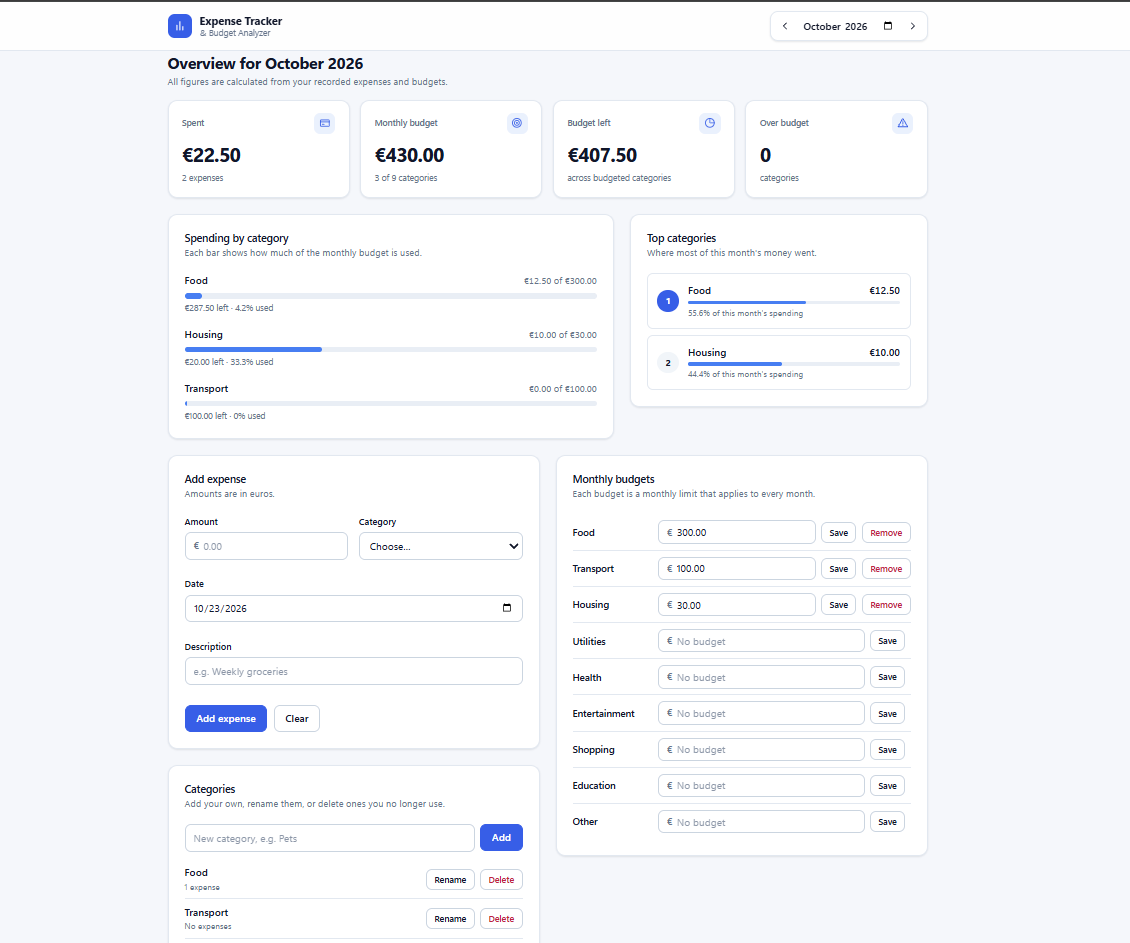
\includegraphics[width=0.9\textwidth]{01-dashboard.png}
%     \caption{Dashboard for one month: summary cards, spending by
%     category against each budget (one category over budget), and the
%     top categories.}
%     \label{fig:dashboard}
% \end{figure}

\textit{Screenshot to be added.}

\subsection{Screenshot 2: Automated Test Results}

% Upload screenshots/04-tests.png to Overleaf, then uncomment.
% \begin{figure}[htbp]
%     \centering
%     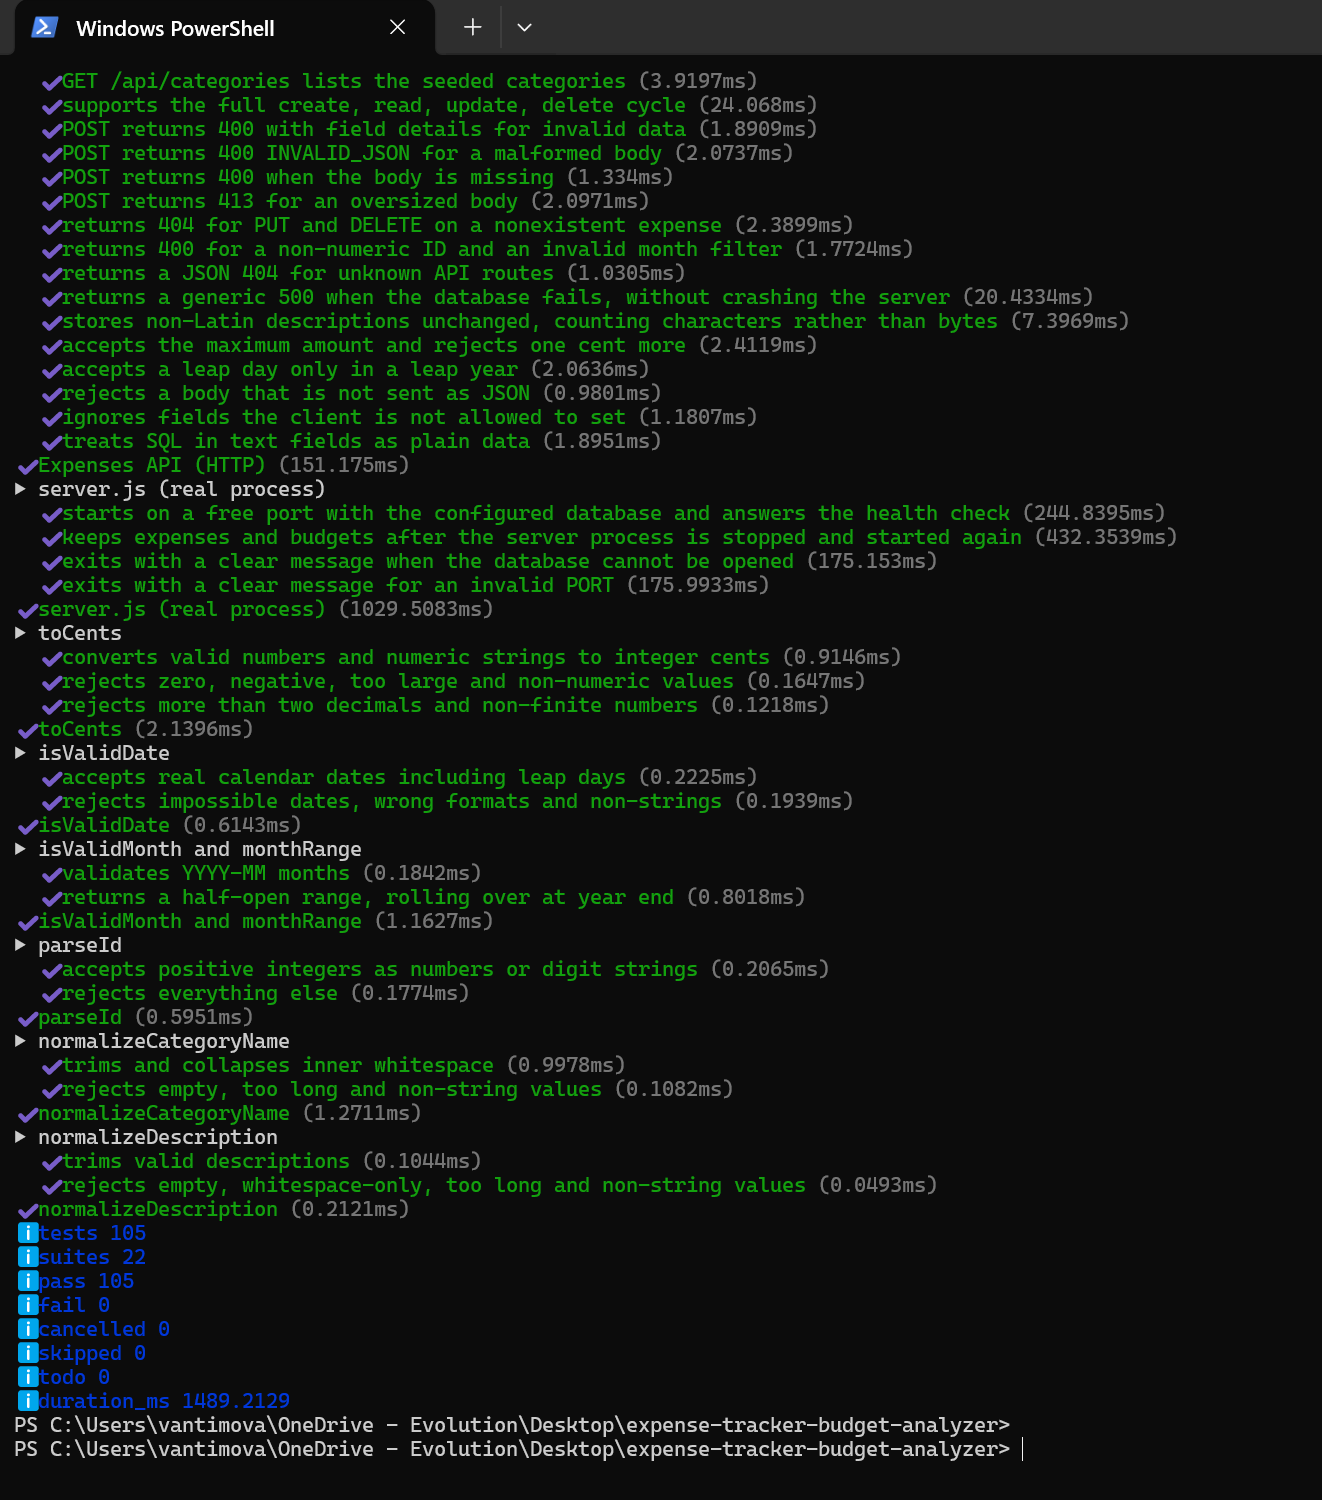
\includegraphics[width=0.9\textwidth]{04-tests.png}
%     \caption{Output of \texttt{npm test}: all automated unit and HTTP
%     integration tests pass.}
%     \label{fig:tests}
% \end{figure}

\textit{Screenshot to be added.}

% Optional third screenshot: 02-expense-management.png
% (editing an expense or the delete confirmation dialog).

% ==================================================
% 6. REPOSITORY AND CONCLUSION
% ==================================================

\section{Repository and Conclusion}

\subsection{GitHub Repository}

The source code, tests, development log, and this report are available
at:

\repolink

\subsection{Conclusion}

% TODO: review and update after the final verification.
The completed system lets a user record, edit, and delete expenses,
manage their own categories, set monthly category budgets, and see
accurate monthly totals, budget usage, and top categories on a
responsive dashboard, with all data stored in SQLite. One hundred and
five automated tests and a 37-step automated browser check confirmed the
main functionality at the time of writing.

The project showed that an AI coding assistant is most effective when
the work is divided into small, approved steps and every claim is
checked against real output. Planning before coding, keeping a
development log, and asking the assistant to prove that its tests can
fail were more valuable than generating large amounts of code quickly.

\end{document}
